\section{The Standard Model Lagrangian}

The Lagrangian which describes the Standard Model, denoted $\mathcal{L}_{\text{\emph{SM}}}$, can, then, be considered a sum of a series of lesser Lagrangians. $\mathcal{L}_{\text{\emph{SM}}}$ can be divided into sectors in several ways, according to the needs of the author \cite{srednicki,wikism}. For this work, the sectors of the Standard Model shall be defined as follows,
\[\mathcal{L}_{\text{\emph{SM}}}=\mathcal{L}_{\text{\emph{EW}}}+\mathcal{L}_{\text{\emph{QCD}}}+\mathcal{L}_{H},\]
into sectors describing the electroweak part $\mathcal{L}_{\text{\emph{EW}}}$, the QuantumChromoDynamics part $\mathcal{L}_{\text{\emph{QCD}}}$ and the Higgs part $\mathcal{L}_{\text{\emph{H}}}$.

The electroweak Lagrangian can be expanded to read as follows:
\[\mathcal{L}_\text{\emph{EW}}=-\ono4W^i_{\mu\nu}W_i^{\mu\nu}-\ono4B_{\mu\nu}B^{\mu\nu}+\sum_\psi\bar\psi\gamma^\mu \left(i\partial_\mu-{1\over2}g^\prime Y_\mathrm{W}B_\mu-{1\over2}g\sigma^a W^a_\mu\right)\psi,\]
where $W^i_{\mu}$ and $B_{\mu}$ are the four ($i$ runs from 1 to 3) gauge fields of electroweak theory and $W^i_{\mu\nu}$ and $B_{\mu\nu}$ are their field strength tensors, the $\phi$ sum is over all left--handed fermionic (lepton and quark) fields, $\gamma_{\mu}$ is the Dirac matrices, $g$ and $g'$ are the coupling strengths of the theory, $Y_W$ is the weak hypercharge associated with the fermionic field and $\sigma_i$ are the Pauli matrices. The terms for right--handed fermions have been omitted.

The physical $W^\pm_\mu$, $Z^0_\mu$ and $A_\mu$ fields, which manifest as the W and Z bosons and the photon, respectively, arise as mixtures of the gauge fields:
\(\begin{aligned}
W_\mu^\pm&=\ono{\sqrt{2}} W^1_\mu\mp iW^2_\mu\\
Z^0_\mu&=W^3_\mu\cos \theta_W-B_\mu\sin \theta_W\\
A_\mu&=W^3_\mu\sin\theta_W+B_\mu\cos\theta_W,
\end{aligned}\label{tophys}\)
where $\theta_W$ is the Weinberg mixing angle, an empirically determined parameter of the model. It also relates the coupling strengths to the electromagnetic coupling constant $e$ though
\[e=g'\cos\theta_W=g\sin\theta_W.\]

Applying the relations in eqs.~\eqref{tophys} allows us to rewrite $\mathcal{L}_{\text{\emph{EW}}}$ to a form that depends solely on these physical fields. Focusing on terms that depend on
\[F_{\mu\nu}=\partial_\mu A_\nu - \partial_\nu A_\mu,\]
the electromagnetic field strength tensor, that come from just the first two terms in $\mathcal{L}_{\text{\emph{EW}}}$, produces
\(\mathcal{L}_{\text{\emph{EW}}}=-\ono4 F^{\mu\nu}F_{\mu\nu}+ie F^{\mu\nu}W^{+}_\mu W^{-}_\nu+\cdots\label{ewfmn}\)
The first of these terms describes the propagation of the $A_\mu$ field from one configuration to another, or, in more immediate terms, the propagation of photons through space. Fourier--transforming to momentum space allows us to write the action for this term as
\(S_{\textit{EW}}=-\ono2\int\frac{d^4k}{(2\pi)^4}\tilde A_\mu(k)k^2\tilde A_\nu(-k)+\cdots,\)
implying that the photon propagator in momentum space is
\(\Delta(k)=\ono{k^2-i\epsilon},\label{phoprop}\)
assuming that momentum conservation is imposed. Here, the modification of the denominator by $i\epsilon$ is included to avoid the pole at $k=0$. This particular way of dealing with poles in the integration of the propagators is due to Richard Feynman, making this the Feynman propagator.

Also due to Richard Feynman is the notion that the terms in the Lagrangian can be represented graphically.

\section{Feynman diagrams}
We represent the photon propagator given in eq.~\eqref{phoprop} graphically as shown in fig.~\ref{phoprop}.

\begin{figure}[hbtp]
\begin{minipage}[c]{.69\textwidth}\centering\footnotesize
\begin{tikzpicture}
\draw[decorate, decoration={snake}] (0,0) -- node[midway,above] {$\gamma$} (2,0) ;
\node[right] at (3,0) {$ = \dfrac{1}{k^2-i\epsilon}$};
\end{tikzpicture}
\end{minipage}\hfill
\begin{minipage}[c]{.3\textwidth}
\caption{Feynman rule for the photon propagator.}
\label{phoprop}
\end{minipage}
\end{figure}

The second term in eq.~\eqref{ewfmn} describes an interaction between the photon and the $W$ bosons, the graphical representation of which is given in fig.~\ref{wwgam}.

\begin{figure}[htbp]
\begin{minipage}[b]{.69\textwidth}\centering\footnotesize
\begin{tikzpicture}
\draw[decorate, decoration={snake, pre=lineto, pre length=5pt}] (0,0) -- +(1.5,0) node[right] {$\gamma$};
\draw[decorate, decoration={snake, pre=lineto, pre length=5pt}](0,0) -- +(240:1.5) node[left] {$W^{+}$};
\draw[decorate, decoration={snake, pre=lineto, pre length=5pt}](0,0) -- +(120:1.5) node[left] {$W^{-}$};
\node[right] at (3,0) {$= ie$};
\end{tikzpicture}
\end{minipage}\hfill
\begin{minipage}[b]{.3\textwidth}
\caption{Feynman rule for the $\gamma W^{+}W^{-}$ coupling.}
\label{wwgam}
\end{minipage}
\end{figure}

The full propagators for the remaining fields require the introduction of the Higgs Lagrangian, which gives the mass terms for those fields. The relevant terms from the Higgs Lagrangian, in terms of physical fields, as given in eq.~\eqref{tophys}, to get the terms
\(\mathcal{L}_H=-\frac{g^2v^2}{4}W^{+\mu}W^{-}_\mu-\frac{g^2v^2}{8\cos\theta_W}Z^\mu Z_\mu,\)
where $v/\sqrt{2}$ is the vacuum expectation value of the Higgs field, given the correct Gauge transformation. From this, we identify the mass terms
\(m_W=\frac{g^2v^2}{2},\qquad m_Z=m_W\cos\theta_W.\)

Including the mass terms in the action for, say, a free Z boson and Fourier--transforming gives us
\[S_Z=?\int\frac{d^4k}{(2\pi)^4}\tilde Z_\mu(k)[k^2-m^2]\tilde Z\nu(-k) +\cdots,\]
leading to the more general form of the Feynman propagator,
\(\Delta(k)=\ono{k^2-m^2-i\epsilon},\)
which is the factor associated with the remaining electroweak propagators, and the Higgs propagator, which are drawn as shown in figure~\ref{ewprops}, along with the gluon propagator produced by $\mathcal{L}_\textit{QCD}$, for completeness.

\begin{figure}[hbtp]
\begin{minipage}[b]{.69\textwidth}
\centering\footnotesize
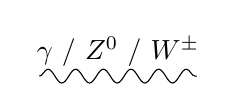
\begin{tikzpicture}
\draw[decorate, decoration={snake}] (0,0) -- node[above] {$\gamma$ / $Z^0$ / $W^\pm$} (2,0);
\end{tikzpicture}
\hspace{5em}
\begin{tikzpicture}
\draw (0,0) -- node[midway] {\tikz\draw[-triangle 45] (0,0) -- (.1,0);} node[midway,above] {$\ell$ / $\nu$ / $q$} (2,0);
\end{tikzpicture}
\vspace{1em}

\begin{tikzpicture}
\draw[dashed] (0,0) -- node[above] {$h$} (2,0);
\end{tikzpicture}
\hspace{5em}
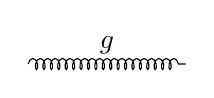
\begin{tikzpicture}
\draw[decorate, decoration={coil,amplitude=2pt, segment length=2.68pt}] (0,0) -- node[above] {$g$} (2,0);
\end{tikzpicture}
\end{minipage}
\hfill
\begin{minipage}[b]{.3\textwidth}
\caption{Showing how line shapes and SM particles are associated.}\label{ewprops}
\end{minipage}
\end{figure}

In fig.~\ref{ewprops}, the notion that antiparticles are time--reversed particles is introduced, as indicated by the direction of the arrows.

The remainder of $\mathcal{L}_\textit{EW}$ gives rise to couplings of the types shown in fig.~\ref{restew}. For brevety, we do not show a complete listing of Feynman rules, only a condensed overview of possible vertices. For a complete listing, see eg. \cite{allfeynrules}. The couplings introduced by the QCD and Higgs sectors are given in figure~\ref{othercoups}.

\begin{figure}[hbtp]\centering {\footnotesize
\begin{tikzpicture}
\draw[decorate, decoration={snake, pre=lineto, pre length=5pt}] (0,0) -- +(1.5,0) node[right] {$Z$};
\draw[decorate, decoration={snake, pre=lineto, pre length=5pt}](0,0) -- +(240:1.5) node[left] {$W^{+}$};
\draw[decorate, decoration={snake, pre=lineto, pre length=5pt}](0,0) -- +(120:1.5) node[left] {$W^{-}$};
\end{tikzpicture}\hspace{2em}
\begin{tikzpicture}
\draw[decorate, decoration={snake, pre=lineto, pre length=5pt}] (0,0) -- +(1.5,0) node[right] {$Z/\gamma$};
\draw[](0,0) -- node[midway,sloped] {\tikz\draw[-triangle 45] (0,0)--(-.1,0);} +(240:1.5) node[left] {$f$};
\draw[](0,0) -- node[midway,sloped] {\tikz\draw[-triangle 45] (0,0)--(.1,0);} +(120:1.5) node[left] {$f$};
\end{tikzpicture}\hspace{2em}
\begin{tikzpicture}
\draw[decorate, decoration={snake, pre=lineto, pre length=5pt}] (0,0) -- +(1.5,0) node[right] {$W^\pm$};
\draw[](0,0) -- node[midway,sloped] {\tikz\draw[-triangle 45] (0,0)--(-.1,0);} +(240:1.5) node[above left] {$\nu,\ell$};
\draw[](0,0) -- node[midway,sloped] {\tikz\draw[-triangle 45] (0,0)--(.1,0);} +(120:1.5) node[above left] {$\ell,\nu$};
\draw (0,0) +(240:1.5) node[below left] {$u,d$} (0,0) +(120:1.5) node[below left] {$d,u$};
\end{tikzpicture}\hspace{2em}
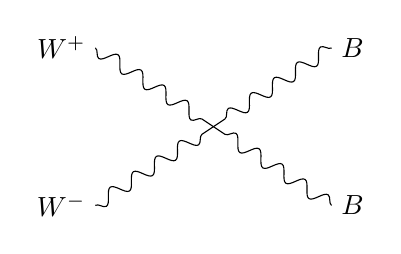
\begin{tikzpicture}
\draw[decorate, decoration={snake, pre=lineto, pre length=5pt}](0,0) -- (-1.5,1) node[left] {$W^{+}$};
\draw[decorate, decoration={snake, pre=lineto, pre length=5pt}](0,0) -- (-1.5,-1) node[left] {$W^{-}$};
\draw[decorate, decoration={snake, pre=lineto, pre length=5pt}](0,0) -- (1.5,1) node[right] {$B$};
\draw[decorate, decoration={snake, pre=lineto, pre length=5pt}](0,0) -- (1.5,-1) node[right] {$B$};
\end{tikzpicture}\hspace{2em}
}
%\begin{tikzpicture}
%\draw[decorate, decoration={snake, pre=lineto, pre length=5pt}](0,0) -- node[above] {$B$} %(2,0);
%\end{tikzpicture}

\caption{The Feynman rules of the electroweak Lagrangian, excluding those given in figures \ref{phoprop} and \ref{wwgam}. Here, $B$ may be any electroweak boson ($\gamma$, $Z^0$ or $W^{\pm}$, so long as charge is conserved. $f$ is any fermion, respecting that photons only couple to electrically charged fermions and $\ell,\nu,u,d$ are lepton--neutrino or up--type---down--type quark sets.} \label{restew}
\end{figure}

An advantage of representing the terms of the Lagrangian in this way is that it allows an easy identification and organisation of possible processes, and subsequently deduction of the action that governs the associated transition amplitude. This is because Feynman diagrams are required to conserve momentum and quantum numbers, and each of the elements of a Feynman diagram are directly associated with an element of the governing equation through Feynman rules, such as were given in fig.~\ref{phoprop} and \ref{wwgam}.

For example, with the $f\bar f \rightarrow \gamma$ and the $q$ propagator already introduced, we may assemble the Feynman diagram in fig.~\ref{bornqq2gg} for a $q\bar q \rightarrow \gamma\gamma$ process.

\begin{figure}[hbtp]
\begin{minipage}[b]{.69\textwidth}
\begin{center}\begin{footnotesize}
\begin{tikzpicture} [>=triangle 45]
\draw[>-] (-1,1) -- (0,1);
\draw[->] (0,1) -- (0,0);
\draw[<-] (-1,-1) -- (0,-1) -- (0,0);
\draw (-2,1) node[left] {$q$} -- (-1,1);
\draw (-2,-1)  node[left] {$\bar q$} -- (-1,-1);
\draw[snake=coil,segment aspect=0] (0,1) -- (2,1) node[right] {$\gamma$};
\draw[snake=coil,segment aspect=0] (0,-1) -- (2,-1) node[right] {$\gamma$}; 
\end{tikzpicture}
\end{footnotesize}\end{center}
\end{minipage}\hfill
\begin{minipage}[b]{.3\textwidth}
\caption{A Feynman diagram for a $q\bar q \rightarrow \gamma\gamma$ process.}\label{bornqq2gg}
\end{minipage}
\end{figure}

To evaluate this diagram, we require the Feynman rule for the $f\bar f \rightarrow \gamma$ vertex, given in fig.~\ref{ruleqqgam}

\begin{figure}[hbtp]
\begin{minipage}[b]{.69\textwidth}
\centering\footnotesize
\begin{tikzpicture}
\draw[decorate, decoration={snake, pre=lineto, pre length=5pt}] (0,0) -- +(1,0) node[right] {$\gamma$};
\draw[](0,0) -- node[midway,sloped] {\tikz\draw[-triangle 45] (0,0)--(-.1,0);} +(240:1) node[left] {$f$};
\draw[](0,0) -- node[midway,sloped] {\tikz\draw[-triangle 45] (0,0)--(.1,0);} +(120:1) node[left] {$f$};
\node[right] at (2,0) {$=eQ_f\gamma^\mu$};
\end{tikzpicture}
\end{minipage}\hfill
\begin{minipage}[b]{.3\textwidth}
\caption{Feynman rule for the fermion--fermion--photon coupling. $e$ is the unit charge and $Q_f$ is the charge of the fermion.}\label{ruleqqgam}
\end{minipage}
\end{figure}

The Feynman diagram in fig.~\ref{bornqq2gg} is then equivalent to
\(\frac{e^2Q_q^2\gamma^\mu\gamma^\nu}{k^2-m^2-i\epsilon},\)
where $k$ is the momentum of the internal quark propagator. This relates to the transition amplitude by integrating over all participating momenta, keeping in mind that momenta must be conserved across all propagators and in every vertex.

The couplings introduced by the QCD and Higgs sectors are given in figure~\ref{othercoups}.

\begin{figure}[htbp]
\centering\footnotesize
\begin{tikzpicture}
\draw[decorate, decoration={coil,amplitude=2pt, segment length=2.68pt, pre=lineto, pre length=5pt}] (0,0) -- +(1.5,0) node[right] {$g$};
\draw[](0,0) -- node[midway,sloped] {\tikz\draw[-triangle 45] (0,0)--(-.1,0);} +(240:1.5) node[left] {$q$};
\draw[](0,0) -- node[midway,sloped] {\tikz\draw[-triangle 45] (0,0)--(.1,0);} +(120:1.5) node[left] {$q$};
\end{tikzpicture}\hspace{2em}
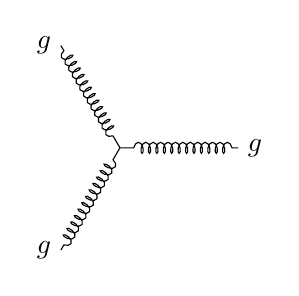
\begin{tikzpicture}
\draw[decorate, decoration={coil,amplitude=2pt, segment length=2.68pt, pre=lineto, pre length=5pt}] (0,0) -- +(1.5,0) node[right] {$g$};
\draw[decorate, decoration={coil,amplitude=2pt, segment length=2.68pt, pre=lineto, pre length=5pt}](0,0) -- +(240:1.5) node[left] {$g$};
\draw[decorate, decoration={coil,amplitude=2pt, segment length=2.68pt, pre=lineto, pre length=5pt}](0,0) -- +(120:1.5) node[left] {$g$};
\end{tikzpicture}\hspace{2em}
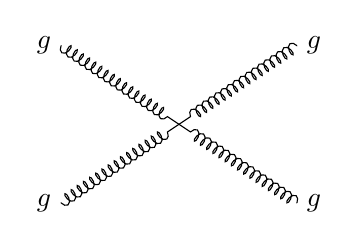
\begin{tikzpicture}
\draw[decorate, decoration={coil,amplitude=2pt, segment length=2.68pt, pre=lineto, pre length=5pt}](0,0) -- (-1.5,1) node[left] {$g$};
\draw[decorate, decoration={coil,amplitude=2pt, segment length=2.68pt, pre=lineto, pre length=5pt}](0,0) -- (-1.5,-1) node[left] {$g$};
\draw[decorate, decoration={coil,amplitude=2pt, segment length=2.68pt, pre=lineto, pre length=5pt}](0,0) -- (1.5,1) node[right] {$g$};
\draw[decorate, decoration={coil,amplitude=2pt, segment length=2.68pt, pre=lineto, pre length=5pt}](0,0) -- (1.5,-1) node[right] {$g$};
\end{tikzpicture}\hspace{2em}
\begin{tikzpicture}
\draw[dashed] (0,0) -- +(1.5,0) node[right] {$h$};
\draw[](0,0) -- node[midway,sloped] {\tikz\draw[-triangle 45] (0,0)--(-.1,0);} +(240:1.5) node[left] {$f$};
\draw[](0,0) -- node[midway,sloped] {\tikz\draw[-triangle 45] (0,0)--(.1,0);} +(120:1.5) node[left] {$f$};
\end{tikzpicture}\hspace{2em}
\begin{tikzpicture}
\draw[dashed] (0,0) -- +(1.5,0) node[right] {$h$};
\draw[decorate, decoration={snake, pre=lineto, pre length=5pt}](0,0) -- +(240:1.5) node[left] {$Z^0$ / $W^\pm$};
\draw[decorate, decoration={snake, pre=lineto, pre length=5pt}](0,0) -- +(120:1.5) node[left] {$Z^0$ / $W^\mp$};
\end{tikzpicture}\hspace{2em}
\begin{tikzpicture}
\draw[dashed] (0,0) -- +(1.5,0) node[right] {$h$};
\draw[dashed](0,0) -- +(240:1.5) node[left] {$h$};
\draw[dashed](0,0) -- +(120:1.5) node[left] {$h$};
\end{tikzpicture}\hspace{2em}
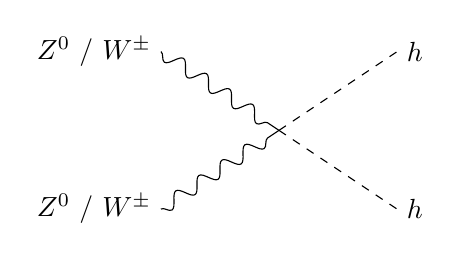
\begin{tikzpicture}
\draw[decorate, decoration={snake, pre=lineto, pre length=5pt}](0,0) -- (-1.5,1) node[left] {$Z^0$ / $W^\pm$};
\draw[decorate, decoration={snake, pre=lineto, pre length=5pt}](0,0) -- (-1.5,-1) node[left] {$Z^0$ / $W^\pm$};
\draw[dashed](0,0) -- (1.5,1) node[right] {$h$};
\draw[dashed](0,0) -- (1.5,-1) node[right] {$h$};
\end{tikzpicture}\hspace{2em}
\begin{tikzpicture}
\draw[dashed](0,0) -- (-1.5,1) node[left] {$h$};
\draw[dashed](0,0) -- (-1.5,-1) node[left] {$h$};
\draw[dashed](0,0) -- (1.5,1) node[right] {$h$};
\draw[dashed](0,0) -- (1.5,-1) node[right] {$h$};
\end{tikzpicture}\hspace{2em}
\caption{Couplings introduced in $\mathcal{L}_\textit{QCD}$ and $\mathcal{L}_H$.}\label{othercoups}
\end{figure}

With these couplings in the mix, we can additionally construct the diagrams with $\gamma\gamma$ final states in figure~\ref{hiorder}.

\begin{figure}[hbtp]
\begin{minipage}[b]{.49\textwidth}
\begin{center}\begin{footnotesize}
\begin{tikzpicture} [>=triangle 45,scale=.8]
\draw[>-] (1,1) node[below]{$q$} -- (2,1);
\draw[decorate, decoration={coil,amplitude=2pt, segment length=2.68pt}] 
    (-2,1) node[left]{$g$} -- (0,1) ;
\draw[decorate, decoration={coil,amplitude=2pt, segment length=2.68pt}] 
    (-2,-1) node[left]{$g$} -- (0,-1); 
\draw[<-] (1,-1) node[above]{$\bar q$} -- (2,-1);
\draw (0,1) -- (1,1);
\draw (0,-1) -- (1,-1);
\draw[-<] (0,1) -- (0,0);
\draw (0,0) -- (0,-1);
\draw[->] (2,1) -- (2,0);
\draw (2,0) -- (2,-1);
\draw[decorate, decoration={snake}] (2,1) -- (4,1) node[right]{$\gamma$};
\draw[decorate, decoration={snake}] (2,-1) -- (4,-1) node[right]{$\gamma$};
\end{tikzpicture}
\end{footnotesize}\end{center}
\end{minipage}\hfill
\begin{minipage}[b]{.49\textwidth}
\centering\footnotesize
\begin{tikzpicture}[scale=.7]
\draw[dashed] (0,0) node[left] {$h$} -- (2,0);
\draw (2,0) -- node[midway,sloped] {\tikz\draw[-triangle 45] (0,0)--(.1,0);} (4,1) --
    node[midway,sloped] {\tikz\draw[-triangle 45] (0,0)--(.1,0);} (4,-1) --
    node[midway,sloped] {\tikz\draw[-triangle 45] (0,0)--(.1,0);} (2,0);
\node at (3.3,0) {$f$};
\draw[decorate, decoration={snake, pre=lineto, pre length=5pt}] (4,1) -- (6,1) node[right] {$\gamma$};
\draw[decorate, decoration={snake, pre=lineto, pre length=5pt}] (4,-1) -- (6,-1) node[right] {$\gamma$};
\end{tikzpicture}
\end{minipage}
\caption{Single loop level Feynman diagrams with $\gamma\gamma$ final states.}\label{hiorder}
\end{figure}

Both these diagrams introduce a new complication, in that the internal loops contain a momentum which is not fixed by momentum conservation in the vertices to external momenta. Thus, the momentum integration on this diagram will diverge. There exist well defined procedures for renormalising the contributions from these loop level diagrams, however, as this requires the development of next--to--leading order methods, we will consider them beyond our scope. We will in any case not be calculating contributions from higher than leading order diagrams directly.

The rightmost diagram in fig.~\ref{hiroder} is one of the decay modes of the Higgs boson. As such, the invariant mass of the resulting photon pair will tend to distribute itself around the Higgs boson mass. In fact, this process was one of the main areas of focus in the recent search for the Higgs boson. This distribution of invarant masses, we will see in the following, is quite different from the signature of the event that are the subject of the present search. Thus, the contribution from this diagram will not figure in the analysis to follow.